% Idea general

% \begin{itemize}
%     \item Parser C3D
%     \item Entorno Bevy
%     \item creación configuraciones (toml)
% \end{itemize}


\chapter{Desarrollo} \label{sec:cap3}


\noindent Este proyecto se ha llevado a cabo en diferentes etapas. En un comienzo, se trabaja con un fichero C3D capturado por las cámaras de INEF, con el sistema de captura de datos de la marca Vicon explicado en el \autoref{sec:cap2}. Estos datos de entrada consisten en una grabación a 240 Hz de un \textit{swing} de golf \footnote{Un swing de golf es la acción mediante la cual los jugadores golpean la pelota en este deporte \autocite{GolfSwing2025}}. Una representación del \textit{swing} en el entorno actual es:

\todo{Figura del swing en el entorno de Enrique}

\begin{figure}[H]
  \centering
  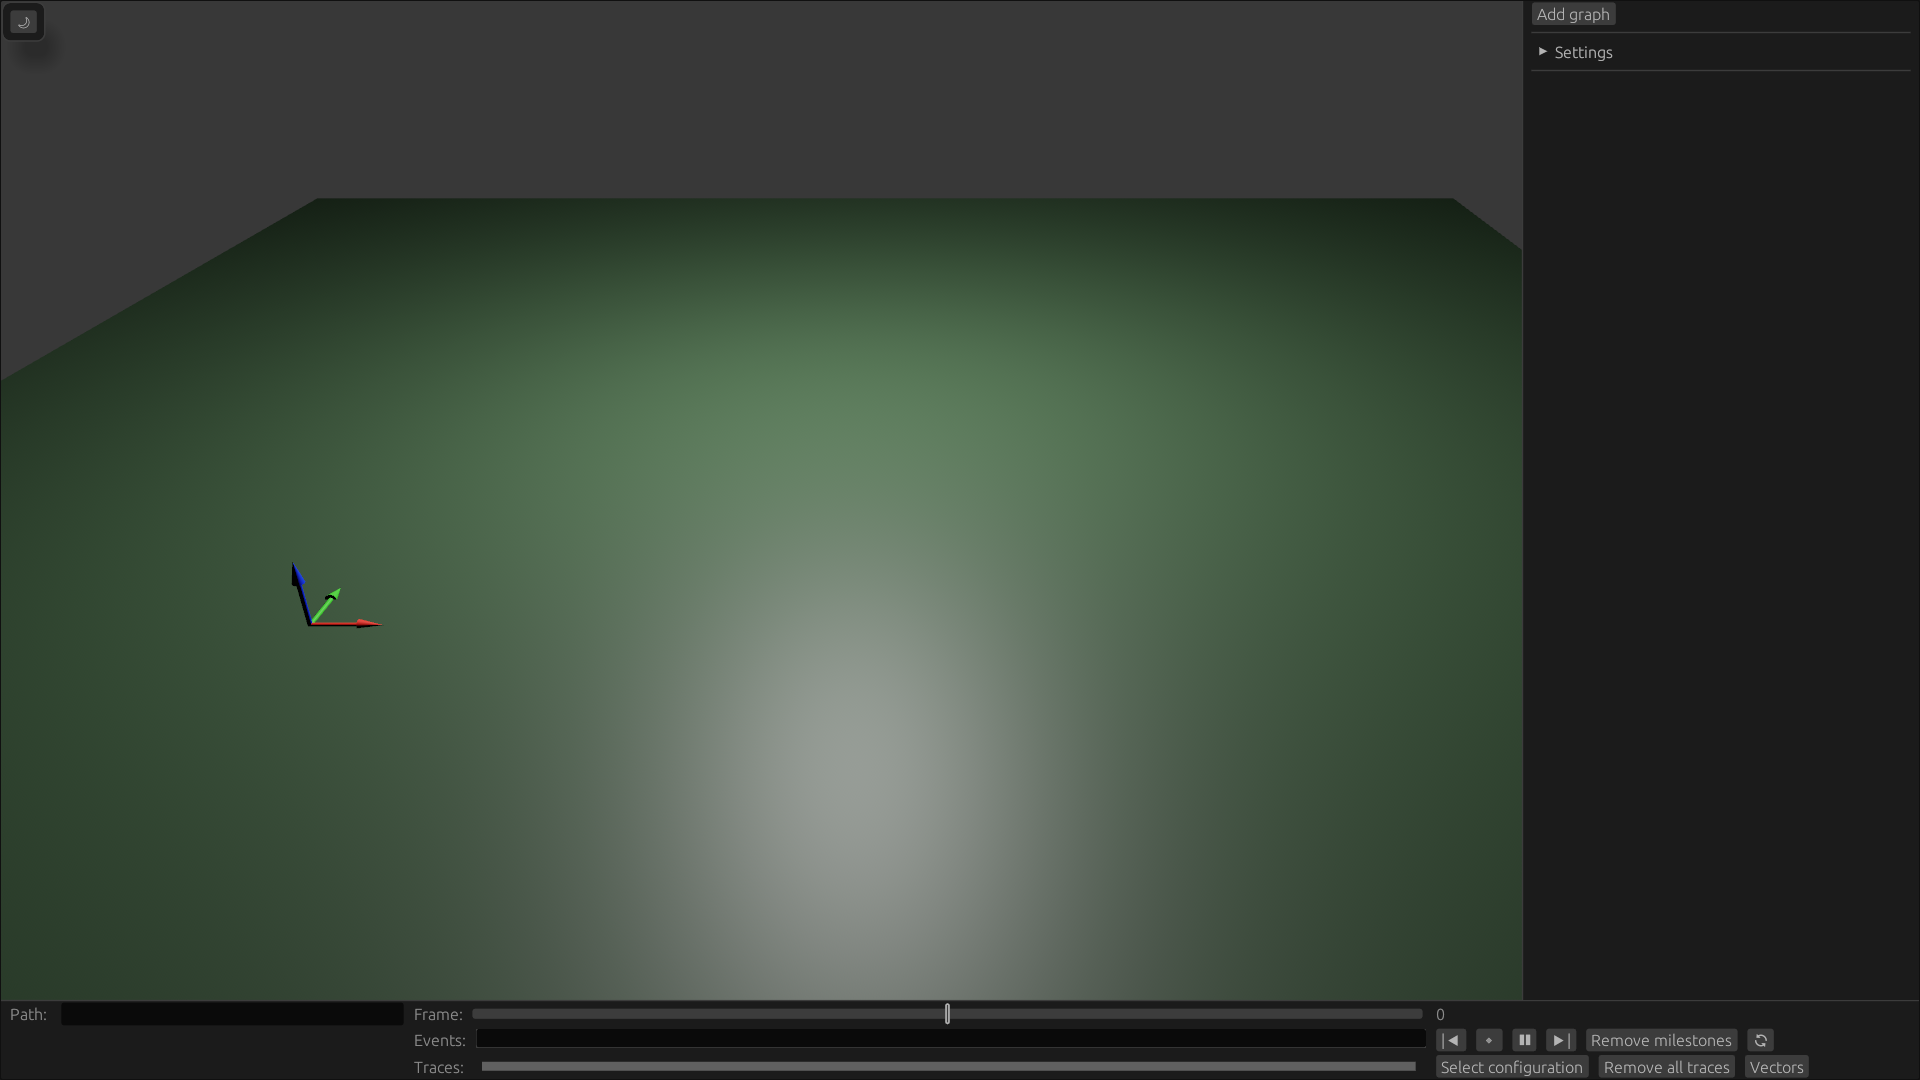
\includegraphics[width=\textwidth]{imagenes/entorno3D.png}
  \caption{Entorno 3D creado con Bevy}
  \label{fig:entorno3D}
\end{figure}